\section{Methods}

\subsection{Rosetta scoring functionality and relevant score functions}\marginnote{This needs to be expanded. Similar to the background document.}
Rosetta uses multiple scoring functions for evaluating macromolecule structures, called poses, in different contexts.
Each score function is a weighted sum of scoring terms that describe some energetic property of the pose.
These energy terms are either physically or statistically derived and may be functions of one or two atoms or residues.
The individual weights, $W_x$, on each energy term are typically fit using a special protocol called OptE\cite{leaver-fay_chapter_2013}.

The Rosetta scoring function can be expressed as in equation \ref{equ:rosetta_sum_of_terms}, where \textit{n} is the total number of residues, $W_{x}$ is the weight on energy term \textit{x} (eg.\ \textit{fa\_rep}, \textit{fa\_sol}, etc.), $E_{x,i}$ is the energy for energy term \textit{x} for the residue at position \textit{i}.

\begin{equation}
  \label{equ:rosetta_sum_of_terms}
  E_{\text{pose}} = \sum_{i}^{n_{\text{res}}} W_{x} E_{x,i} + ... + W_{y} E_{y,i}
\end{equation}

% I hate the phrase "designed for general purpose protein evaluation" but I'm not sure of a better successor. Really, I just want to say that it's only compatible with canonical amino acids...
Rosetta protocols most frequently use the scoring function \textit{talaris2013}, which was designed for general purpose protein evaluation using canonical amino acids\cite{leaver-fay_chapter_2013}.
It consists of the score terms \textit{fa\_atr}, \textit{fa\_rep}, \textit{fa\_sol}, \textit{fa\_elec}, \textit{fa\_intra\_rep}, \textit{pro\_close}, \textit{hbond\_sr\_bb}, \textit{hbond\_lr\_bb}, \textit{hbond\_bb\_sc}, \textit{hbond\_sc}, \textit{dslf\_fa13}, \textit{rama}, \textit{omega}, \textit{fa\_dun}, \textit{p\_aa\_pp}, and \textit{ref}.
Full descriptions of these energy terms can be found in \cite{leaver-fay_chapter_2013}.
%optionally include descriptions of these terms here.

The scoring function \textit{mm\_std} is available to model structures that include NCAAs and peptidomimetics, called \cite{renfrew_incorporation_2012}.
The energy terms of this score function are \textit{fa\_atr}, \textit{fa\_rep}, \textit{fa\_sol}, \textit{mm\_lj\_intra\_atr}, \textit{mm\_lj\_intra\_rep}, \textit{mm\_twist}, \textit{pro\_close}, \textit{hbond\_sr\_bb}, \textit{hbond\_lr\_bb}, \textit{hbond\_bb\_sc}, \textit{hbond\_sc}, \textit{dslf\_ss\_dst}, \textit{dslf\_cs\_ang}, \textit{dslf\_ss\_dih}, \textit{dslf\_ca\_dih}, and \textit{unfolded}.
\textit{mm\_std} lacks the statistical potentials used by \textit{talaris2013}, such as \textit{p\_aa\_pp}, which derives from the probability that a given residue type is found at a given point in Ramachandran space.
Since such statistical potentials are not available for NCAAs in general, the molecular mechanics potentials are included to compensate.
Crucially, \textit{mm\_std} replaces \textit{ref} with an explicit energetic model of the unfolded state of each residue, called \textit{unfolded}.

\subsection{The structure of the two-component reference energy}\marginnote{This is the crux of the whole paper. Need the equation.}
The two-component reference energy (TCRE) addresses the aforementioned shortcomings of $unfolded$ by treating the one- and two-body energies of a residue separately.
By evaluating the two-body scoring terms in the context of folded proteins, the TCRE eliminates any bias towards large residues.
By evaluating one body energies in the context of an acetylated, methylamidated dipeptide, the TCRE avoids any context-dependent issues of scoring
Each residue type possesses a one body energy and a two body energy derived from the summed two body scores of its constituent atom types.
The relative weights of those components are free to be optimized.
% I find the below statement far too vague and speculative. -amw
%In addition, the method can be applied to arbitrary peptides and peptidomimetics by dynamically constructing residue reference energies from constituent atomic energies in response to the residue types in use, which allows the method to be extended to theoretically arbitrary molecules in Rosetta.

\subsection{Generating per-atom-type two-body energy distributions}
The "two-body" component of the split unfolded energy is derived from examining the distribution of individual two-body scoring terms over all the occurrences of a given atom type in a high quality set of protein structures.
To evaluate the effect of our choice of "atom type" set, we examined both the modified CHARMM atom type set used by Rosetta\cite{leaver-fay_chapter_2011,bernard_charmm_1983} and the molecular mechanics (MM)-based atom types\cite{renfrew_incorporation_2012}. % Doug--these are also CHARMM derived, right? How should we phrase the distinction?
As limiting cases, we considered elemental types, where all atoms of the same element are alike, as well as unique atom types, where every atom of every residue type is treated differently.
The Top8000 benchmark set of high quality structures\cite{lovell_structure_2003} provides around $10^6$ examples of most atom types. These structures were scored with Rosetta using a modified protocol that recorded every inter-atomic energy value for the scoring terms \textit{fa\_atr}, \textit{fa\_rep}, \textit{fa\_sol}, \textit{fa\_elec}, \textit{hbond}, and \textit{dslf\_fa13}.
These inter-atomic energies were evaluated on each example of each atom type, and a measure of centrality was extracted from the resulting distribution.

%Table to illustrate the differences between the atom type sets.
\begin{table}
  \centering
  \caption{The four atom type sets categorize the above examples of carbon atoms commonly found in protein structures quite differently.}
  \label{tab:atypes_example}
  \begin{tabular}{clllll}
    \toprule
    Residue & Atom Name & Elemental Type & Rosetta Type & MM Type & Unique Type\\
    \midrule
    GLY & $\alpha$-Carbon & C & CAbb & CT1 & GLY/2\\
    ALA & $\alpha$-Carbon & C & CAbb & CT1 & ALA/2\\
    ALA & $\beta$-Carbon & C & CH3 & CT3 & ALA/5\\
    ALA & Carboxyl Carbon & C & CObb & C & ALA/3\\
    %Perhaps two more that differentiate Rosetta and MM?
    \bottomrule
  \end{tabular}
\end{table}

We evaluated the mean, median, mode, and Boltzmann-weighted average as central measures for each scoring term.
The median exhibited a slight advantage in sequence recovery benchmarks (FIGURE?!) and was used in all further testing.

\subsection{Atom types only found in NCAAs}
A limited number of atom types found in NCAAs currently implemented in Rosetta are not found in canonical amino acids, and thus cannot be scored using the Top8000 data set.
To obtain expected energy distributions for these atom types, which include e.g. the halogens, we mutated all instances of a canonical residue type to a noncanonical analogue that includes the atom type in question and performed limited rotamer repacking and mimimization to resolve clashes.
We analyzed the resulting scoring term distributions in the same way.
Table \ref{tab:atypes_all} describes the molecular mechanics atom types which had to be evaluated in this way.


%Probably want to trim this to just NCAA atom types and/or move it to the supplement...
\begin{table}
  \centering
  \caption{MM atom types found only in NCAAs for which two body energies were obtained.}
  \label{tab:atypes_all}

  \begin{tabular}{c|l}
    \toprule
    Atom Type & description\\
    \midrule
    BR & bromine\\
    CAP & aromatic carbon in pyridine ring\\
    CE1 & monosubstituted alkene carbon\\
    CE2 & terminal alkene carbon\\
    CF1 & monofluorinated carbon\\
    CF3 & trifluorinated carbon\\
    CL & chlorine\\
    F1 & fluorine on CH$_2$R\\
    F3 & fluorine on CF$_2$R\\
    HE1 & proton on monosubstituted alkene carbon \\
    HE2 & proton on terminal alkene carbon\\
    I & iodine\\
    OE & ether oxygen\\
    \bottomrule
  \end{tabular}
\end{table}


\begin{figure}
  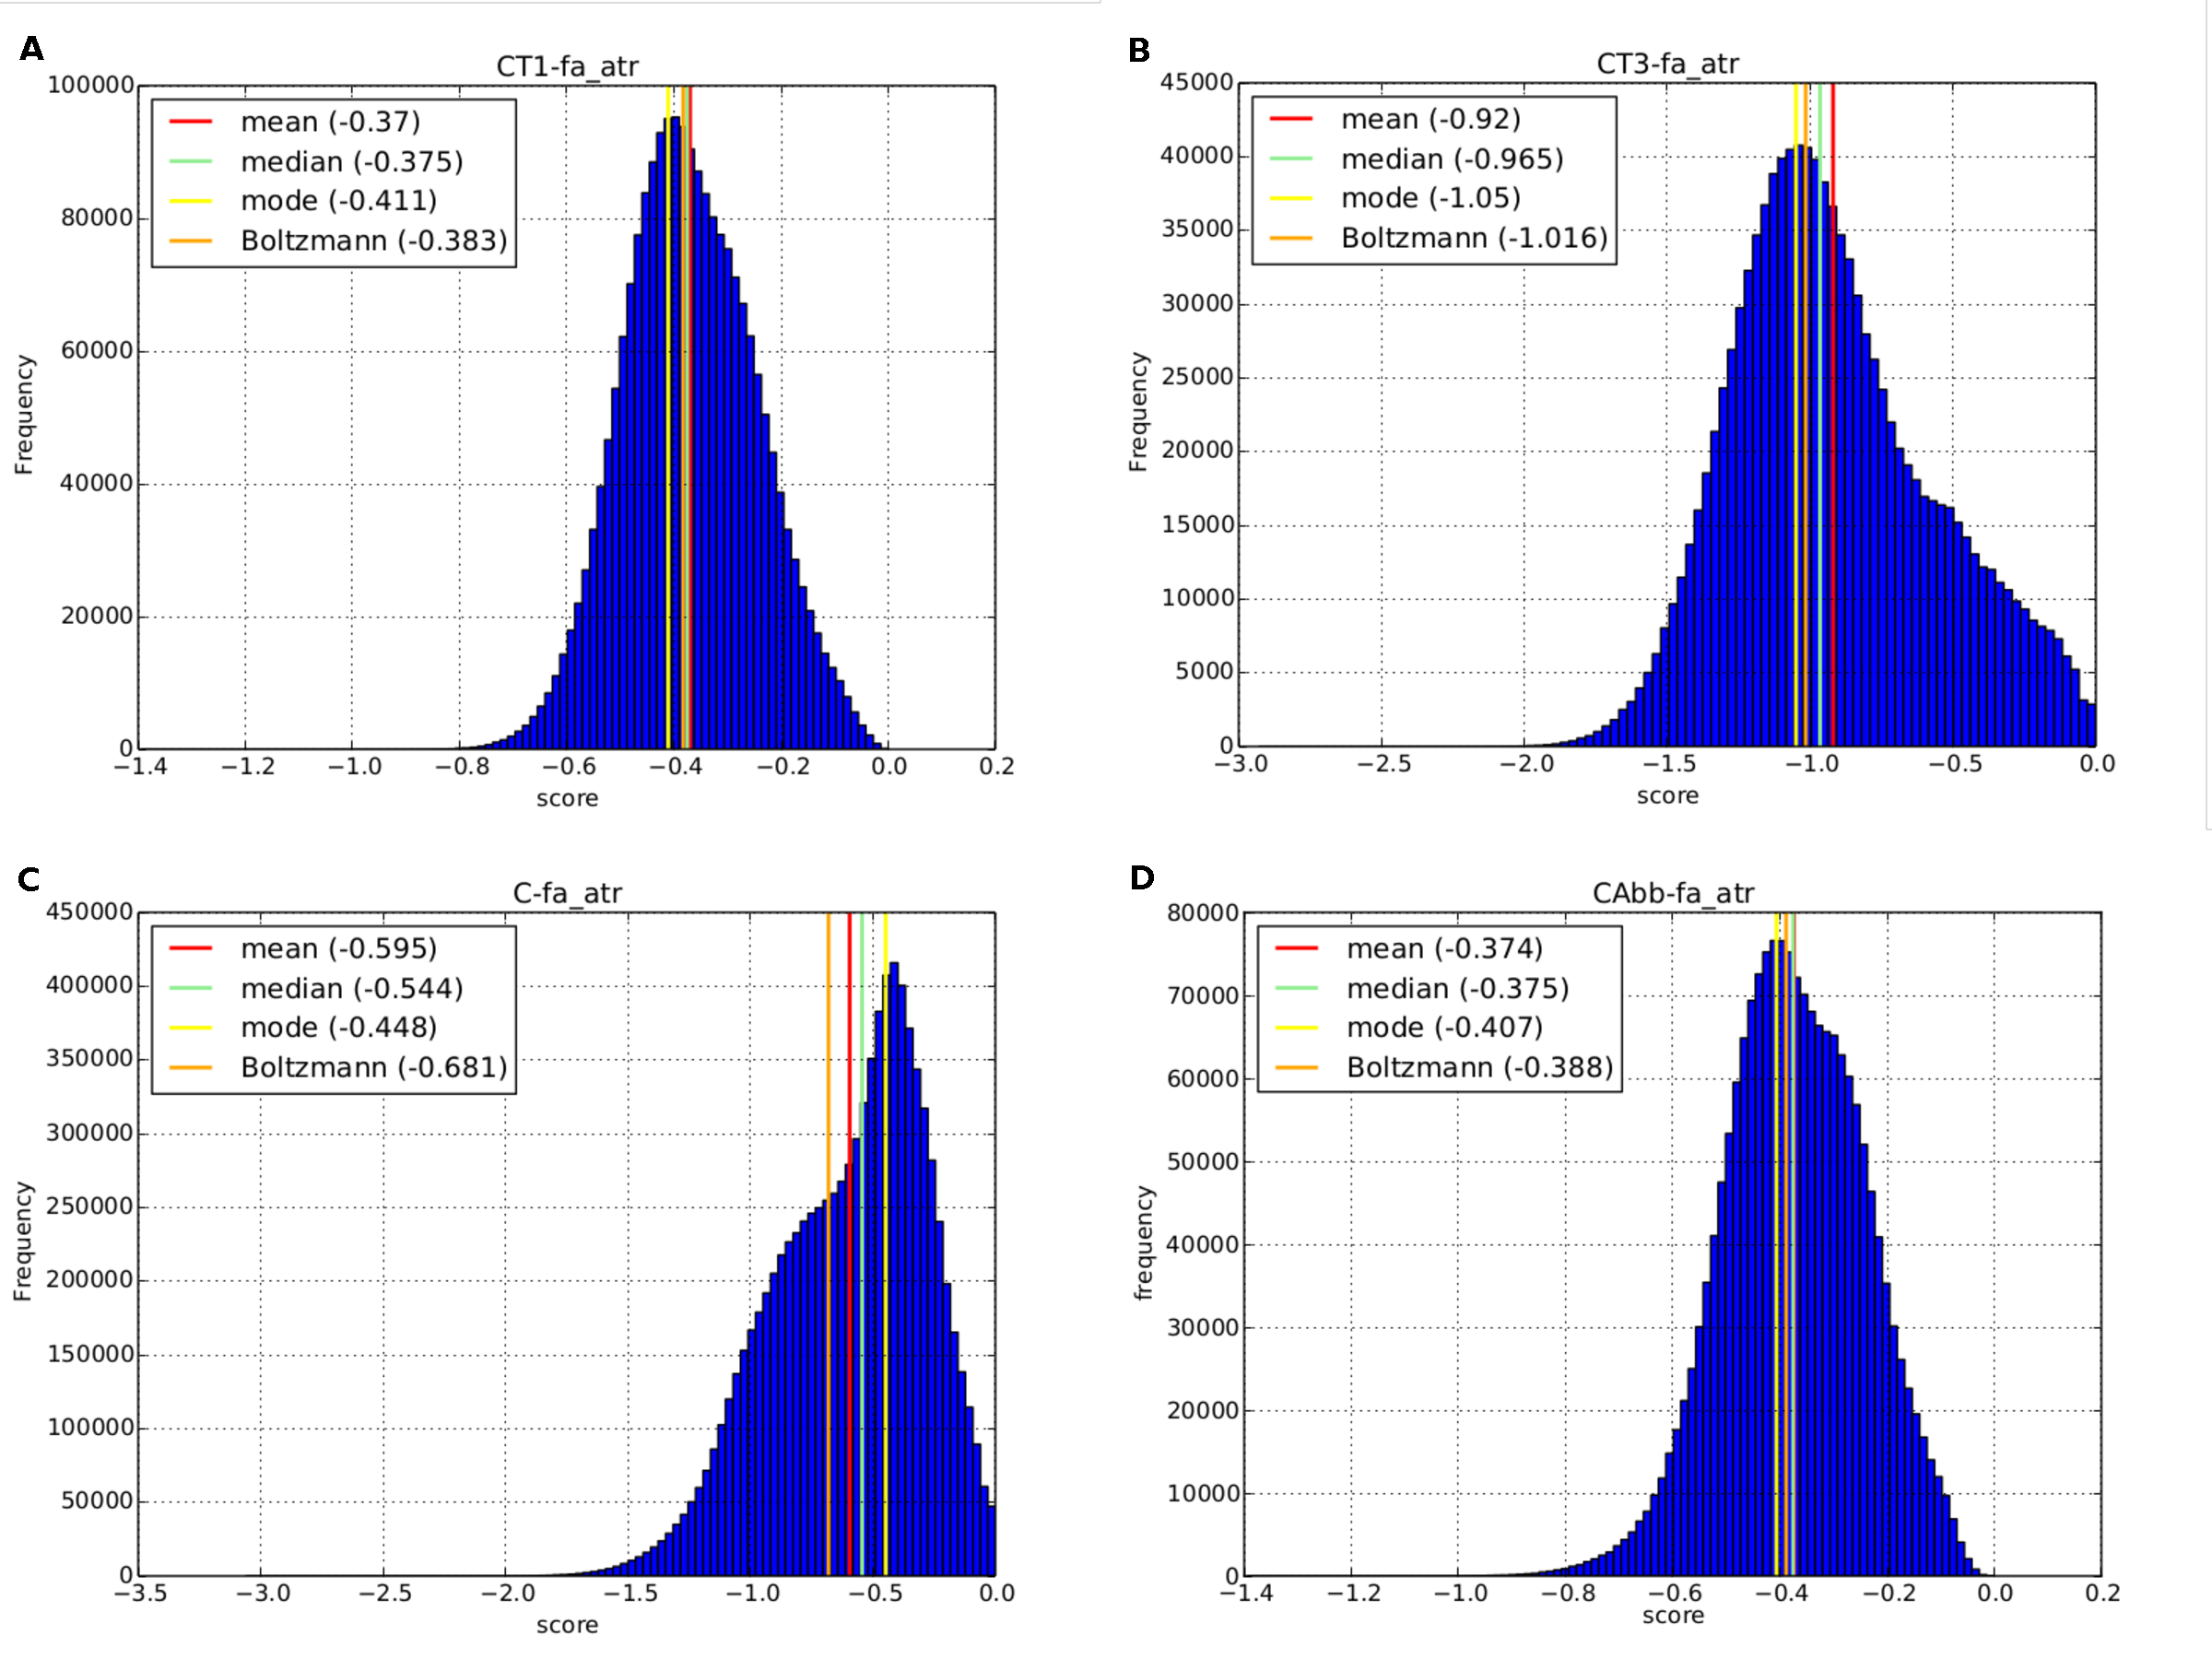
\includegraphics[width=\linewidth]{Figures/atom_energy_distribution_examples.pdf}
  \caption{Example histograms of the \textit{fa\_atr} Lennard-Jones attractive component energy term for several atoms in different atom sets.
    \textbf{A.} The molecular mechanics atom type CT1, a carbon with one hydrogen, and the atom type of the backbone $\alpha$-carbon, among other carbon atoms.
    \textbf{B.} The molecular mechanics atom type CT3, a methyl group, used in several amino acid sidechains.
    \textbf{C.} The elemental atom type C, carbon.
    \textbf{D.} The Rosetta atom type CAbb, the backbone $\alpha$-carbon.
    The median value shown by the green line is the representative value used to construct the amino acid two body energies.}
  \label{fig:tbaedist}
\end{figure}


%\subsection{Formulation of the two component reference energy}
%Our split unfolded energy function is composed of two scoring terms in Rosetta, a one body and a two body component.
%During scoring, each of these terms is calculated separately for each residue in the protein, and then weighted and summed similar to each other Rosetta energy term.
%This combined energy term serves to replace the standard Rosetta reference energy function, known as $ref$.
%The formulation of the two component reference energy for a protein, $E_{TCR}$, is thus:

%replaced with a better equation in a figure from Doug's Rosettacon 2014 poster.
%\begin{equation}
%  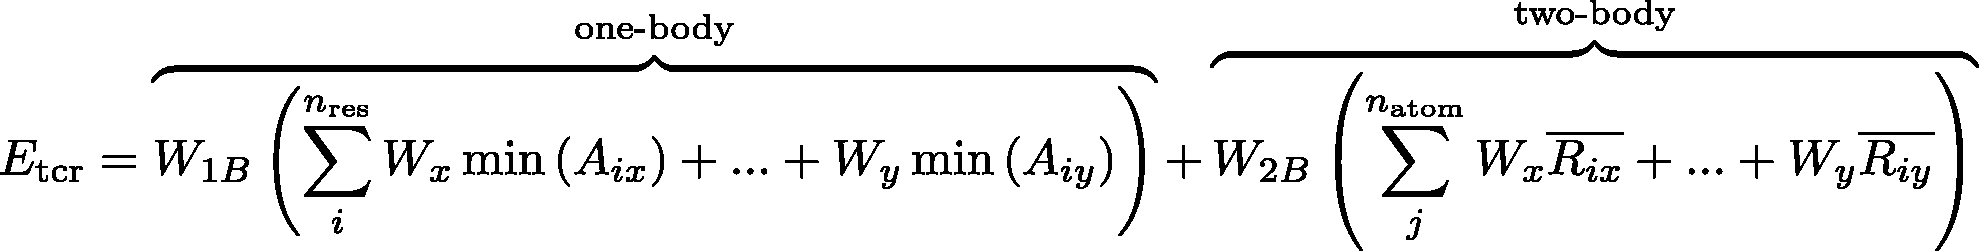
\includegraphics[width=0.9\linewidth]{Figures/tcr_equation.pdf}
%E_{\text{unfolded}} =  W_{1body} \sum_{i}^{n_{\text{res}}} E_{i,1body} +  W_{2body} \sum_{i}^{n_{\text{res}}} E_{i,2body}
%\end{equation}

%Where $W_{1B}$ is the weight placed on the one body term, $W_{2B}$ is the weight placed on the two body term, $min(A_{ix})$ is the minimal value for the one body energy term \textit{x} of the reference energy for residue \textit{i}, and $R_{jx}$ is the median two body energy term \textit{x} for residue \textit{j}.

%\subsection{Calculation of the two body energy term}
%The two body portion of our two component reference energy consists of a sum of the energies of each constitutent atom.
%These atomic energies are calculated from instances of each atom type in the set used appearing in the top8000 data set of high-quality protein crystal structures, as described above.
%These values for each Rosetta score term calculated on a per-atom basis are stored in a lookup table, and per-residue two body unfolded energies are built dynamically as needed during runtime from these atom energy lookups.
%The two body reference energy for the protein is calculated as follows:

%\begin{equation}
%E_{\text{2body}} = W_{2body} \sum_{i}^{n_{\text{res}}} \sum_{j}^{l_{\text{scoreterms}}} W_{j} \sum_{k}^{m_{\text{atoms}}} E_{k}
%\end{equation}

%Where $W_{two-body}$ is the weight value for the two body term, \textit{n} is the total number of residues, \textit{l} is the score terms \textit{fa\_atr}, \textit{fa\_rep}, \textit{fa\_sol}, \textit{fa\_elec}, \textit{hbond}, and \textit{fa\_dslf13} for the \textit{talaris2013} scoring function and the score terms \textit{fa\_atr}, \textit{fa\_rep}, \textit{fa\_elec}, \textit{hbond}, and \textit{fa\_dslf13} for the \textit{mm\_std} scoring function, $W_{j}$ is the weight on score term \textit{j}, \textit{m} is the number of atoms in the residue \textit{i}, and $E_{k}$ is the energy of atom \textit{k} in the two body atom energy lookup table.


\subsection{Determining the single-body reference energy}
The one body component of the reference energy represents the minimum achievable energy of a given residue type for a given scoring function.
We prepended and appended acetyl and N-methylamide capping groups to the residue in question and iterated its backbone dihedral angles in one degree bins, followed by backbone minimization, sidechain repacking, and sidechain minimization.
The lowest energy conformation among those sampled was taken as the ideal conformation for that residue type.
The weighted sum of its intra-residue energies serve as the single-body component of the TCRE.
This process was carried out using the intra-residue scoring terms for both the \textit{talaris2013} score function and the \textit{mm\_std} score function.
For \textit{talaris2013}, the intra-residue terms are \textit{fa\_intra\_rep}, \textit{pro\_close}, \textit{fa\_dun}, \textit{rama}, \textit{omega}, and \textit{p\_aa\_pp}.
For \textit{mm\_std}, the intra-residue terms are \textit{mm\_lj\_intra\_rep}, \textit{mm\_lj\_intra\_atr}, \textit{mm\_twist}, and \textit{pro\_close}.

%During runtime, the one body reference energy of a protein is determined by summing the values thus recorded for each residue type in it's sequence, which is then weighted and summed with the other score terms to produce the total energy of the protein.
%The formulation of the one body term for a given protein is described below.

%\begin{equation}
%E_{\text{1body}} = W_{1body} \sum_{i}^{n_{\text{res}}} \sum_{k}^{j_{\text{scoreterms}}} W_{k} %E_{restype_{i},k}
%\end{equation}

%Where $W_{1body}$ is the one body energy term weight, \textit{n} is the total number of residues, \textit{j} is the set of score terms used to compute the one body energy term for the current score function(either \textit{talaris2013} or \textit{mm\_std}), $W_{k}$ is the weight applied to score term \textit{k} under the energy function in use, and $E_{restype_{i},k}$ is the one body minimal energy value for the score term \textit{k} for the residue type of residue \textit{i} in the protein.


\subsection{Design Benchmarking via Sequence Recovery}
To test the utility of our two component reference energy for protein design, we used the Rosetta native sequence recovery benchmark protocol\cite{leaver-fay_chapter_2013}.
In this protocol, a collection of 41 high-quality protein structures are fully redesigned by Rosetta using a given scoring function.
Two qualities of the scoring function are tested: its ability to recapitulate the native amino acid at each position and its ability to recapitulate overall native amino acid frequencies.
Both metrics describe its ability to design ``natural-like'' protein sequences for a given structure.
To guide analysis, we categorized the twenty canonical amino acids as hydrophobic, polar, positively charged, and negatively charged, since residues in each category response similarly to individual scoring terms.
%These categories were hydrophobic amino acids, consisting of residues valine, isoleucine, leucine, methionine, phenylalanine, glycine, alanine, proline, tryptophan, and tyrosine, polar amino acids, consisting of residues serine, threonine, asparagine, and glutamine, positively charged amino acids, consisting of residues arginine, lysine, and histidine, and negatively charged amino acids, consisting of aspartic acid and glutamic acid.
Using \textit{ref}, the canonical reference energy, \textit{talaris2013} performs much better on hydrophobic amino acids, moderately well on polar amino acids, and much worse on positive and negative amino acids.
%While no benchmark set exists for the design of non-canonical residue types, performance on the canonical residue types should be indicative of performance on NCAA types as well, as these types are treated identically during runtime.
